\chapter{Results of the experiments}
\label{chap:exp}

\section{Flow eviction timeout}
\label{res:eviction-timeout}
\todo{fix plot scaling}

\begin{figure}
    \centering
    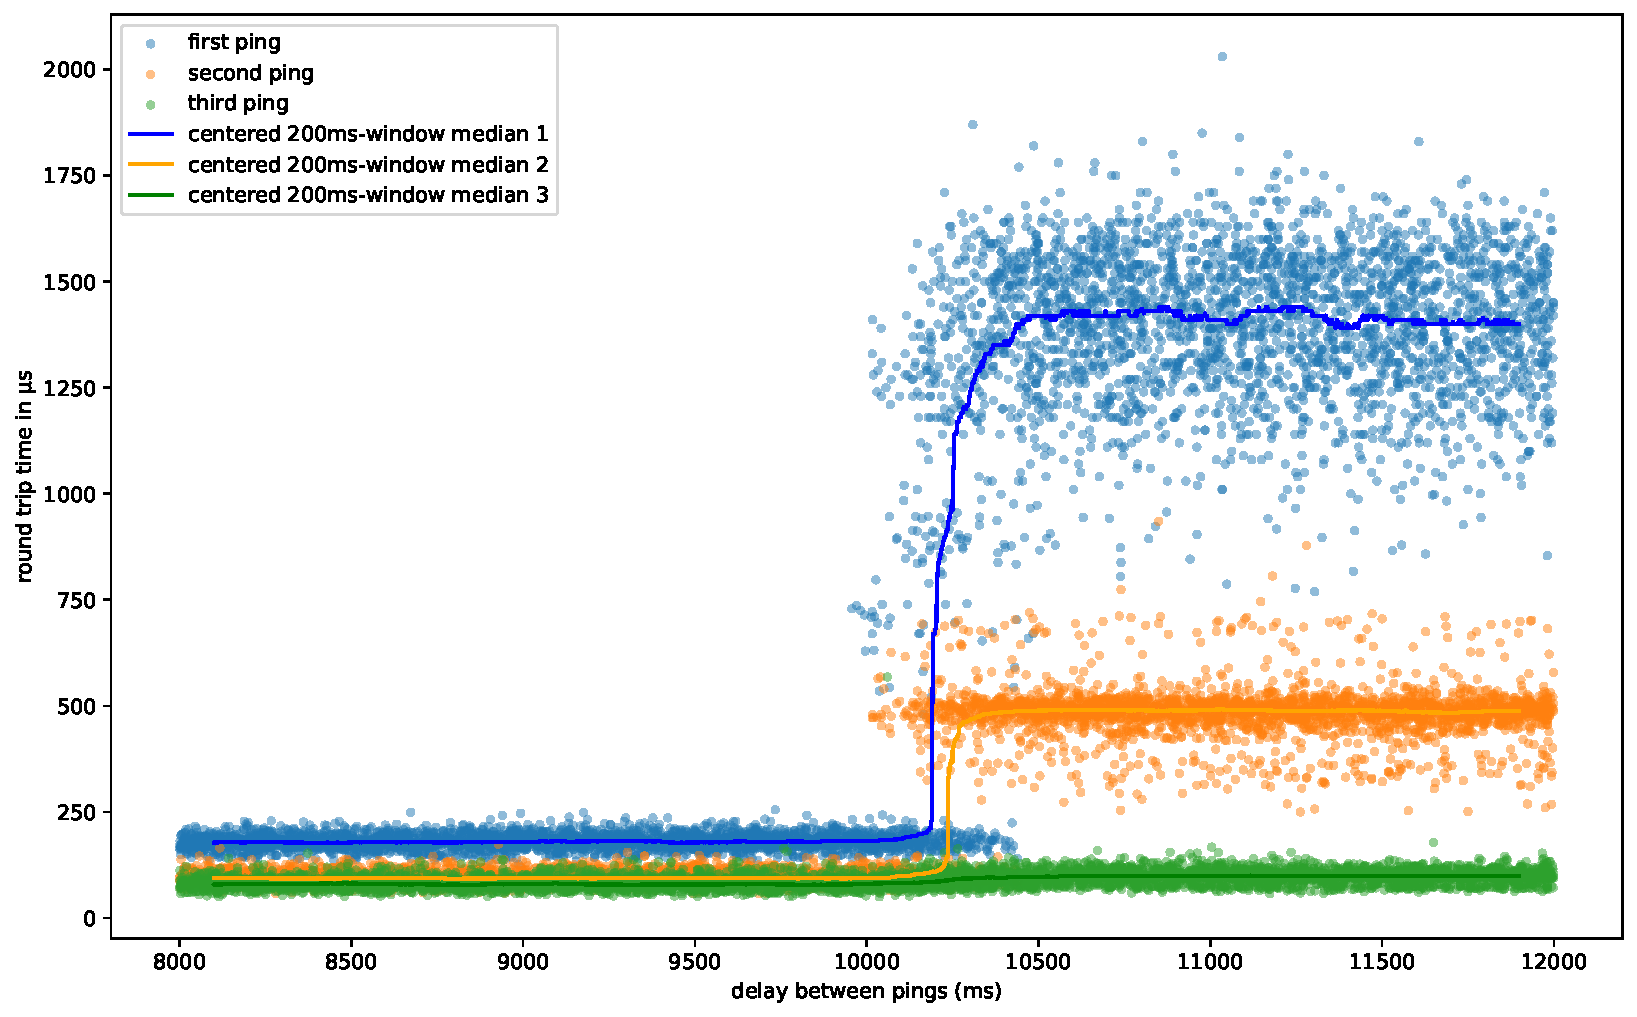
\includegraphics[width=.9\linewidth]{img/randomized_eviction_timeout.pdf}
    \caption{Results of the eviction timeout experiment with cropped outliers}
    \label{fig:plot-eviction-timeout}
\end{figure}

\paragraph{The eviction timeout} The measured latencies of the experiment (\cref{fig:plot-eviction-timeout}) show the flow rule eviction taking effect about $10$ seconds after the last datapath rule installation. The observed value is not exact, but it is probably reasonable to assume the developers chose a nice-looking number. We hypothesize that the noise in the location of the increase is introduced mainly by infrequent eviction checks.

Following these experimental findings, we searched the source code and it specifies exactly $10$ seconds as the default eviction timeout. The experimental findings are consistent with the source code. The default rule timeout defined in the file \ident{ofproto/ofproto.h}:
\begin{verbatim}
#define OFPROTO_MAX_IDLE_DEFAULT 10000 /* ms */
\end{verbatim}

The file \ident{ofproto/ofproto-dpif-upcall.c} contains the code enforcing the timeout in the function \ident{revalidate()}:

\begin{verbatim}
if (kill_them_all || (used && used < now - max_idle)) {
    result = UKEY_DELETE;
}
\end{verbatim}

The eviction is handled by the revalidator threads, which run periodically roughly every 500ms. This confirms our hypothesis about the roughly 500ms spread of the observable timeout effect.

\begin{verbatim}
// in file ofproto/ofproto.h:321
#define OFPROTO_MAX_REVALIDATOR_DEFAULT 500 /* ms */

// in the ofproto/ofproto_dpif_upcall.c:1052
// in function udpif_revalidator()
poll_timer_wait_until(start_time + MIN(ofproto_max_idle,
                                    ofproto_max_revalidator));
\end{verbatim}

\paragraph{Difference in latency below timeout}
\Cref{fig:plot-eviction-timeout} shows a difference between round trip times for the first and second packet even below the eviction timeout. The difference is small, so we assume that this can be caused by CPU caches. We did not investigate this further.

\paragraph{Increase in round trip time of the second ping}
\Cref{fig:plot-eviction-timeout} also shows an increased latency for the second ping after the eviction timeout. We hypothesize that it could be caused by the fixed size flow lookup cache described in \cref{subsec:matching-algo}. The upcall installs the new flow, but the lookup cache is filled only after the first use (i.e. the second packet of the flow, the second ICMP ping). In other words, if we had three packets, their journey through the \ident{openvswitch} module would be as follows:

\begin{enumerate}
    \item A cache miss, followed by a flow table miss. Leads to an upcall and a new flow rule.
    \item A cache miss, which requires a full flow table scan. The cache is filled.
    \item Cache hit.
    \item All consecutive packets hit the cache unless the cache entry is somehow overwritten.
\end{enumerate}

The third RTT measurement behaves as expected by our hypothesis. We shortly experimented with even more consecutive measurements and they were all the same.


\section{Cost of an upcall}
\label{res:upcall-cost}
\todo{this section is not great... Improve...}

\paragraph{Upcall processing cost}
As discussed in \cref{chap:design}, the round trip time increase can be attributed to the cost of upcall processing. In the previous section, we noticed an increased latency with the second RTT measurement, possibly a cache miss in the kernel datapath.  We can estimate the cost of an upcall using this data. We calculated the difference between the first and the second ping measurements and assume the result is the lower bound for the upcall cost. Either our hypothesis about the cache miss is correct. Then the difference would be exactly the time spent processing the upcall. Or, we are wrong and the higher second ping latencies are caused by some additional factor which is not normally present. In that case, the upcall cost would be certainly equal to or higher than our result. We used only the data points with above $10.5$ second delay since the last measurement.

% QT_QPA_PLATFORM=xcb python postprocessing/randomized_eviction_timeout.py results/randomized_eviction_timeout/*.csv
\begin{table}[h!]
    \begin{center}
        \caption{Statistics of measured round trip times when the interval > 10.5 seconds}
        \label{tab:upcall-cost}
        \begin{tabular}{r|S[table-format=4.2]S[table-format=4.2]S[table-format=4.2]}
            & \textbf{First ping RTT} & \textbf{Second ping RTT} & \textbf{Difference} \\
            \hline
            \textbf{\#samples} & 1596 & 1596 & 1596 \\
            \textbf{Mean} & 1399.94 & 483.66 & 916.28 \\
            \textbf{Std} & 162.74 & 59.73 & 154.52\\
            \hline
            \textbf{Min} & 769 & 250 & 149 \\
            \textbf{25th percentile} & 1300 & 467 & 814 \\
            \textbf{Median} & 1410 & 488.0 & 935 \\
            \textbf{75th percentile} & 1520 & 504 & 1031 \\
            \textbf{Max} & 2030 & 878 & 1460 \\
        \end{tabular}
    \end{center}
\end{table}

The mean of the latency difference is within $916.28 \pm 7.59$ \si{\micro\second} with 95\% confidence. 

\paragraph{Comparison to previous results}

We can not directly compare our results with \href{https://developers.redhat.com/articles/2022/02/07/investigating-cost-open-vswitch-upcalls-linux}{Eelco Chaudron's}, because we do not have the same test environment. Under simulated normal conditions, he concluded that the time from the kernel's upcall invocation til the kernel's packet execution is on average $149.83$ \si{\micro\second} ($56446$ samples). Our results are 6x higher. In the same article, he notes:

\begin{quote}
My sample runs have shown what I want to emphasize in this article: The way the upcalls are generated highly influences the outcome of the upcall costs.
\end{quote}

And he shows, that under stress the average upcall cost can be $29367.91$ \si{\micro\second} ($13807$ samples). Therefore, all we can say is that our results are in the range of possible upcalls costs according to his article.

%┌────────────┬───────────────────────────┬─────────────┬─────────────┬───┬─────────────┬──────────────┬──────────────┬─────────────┐
%│ describe   ┆ us_since_last_measurement ┆ us_latency1 ┆ us_latency2 ┆ … ┆ us_latency5 ┆ first_second ┆ second_third ┆ first_third │
%│ ---        ┆ ---                       ┆ ---         ┆ ---         ┆   ┆ ---         ┆ ---          ┆ ---          ┆ ---         │
%│ str        ┆ f64                       ┆ f64         ┆ f64         ┆   ┆ f64         ┆ f64          ┆ f64          ┆ f64         │
%╞════════════╪═══════════════════════════╪═════════════╪═════════════╪═══╪═════════════╪══════════════╪══════════════╪═════════════╡
%│ count      ┆ 1596.0                    ┆ 1596.0      ┆ 1596.0      ┆ … ┆ 1596.0      ┆ 1596.0       ┆ 1596.0       ┆ 1596.0      │
%│ null_count ┆ 0.0                       ┆ 0.0         ┆ 0.0         ┆ … ┆ 0.0         ┆ 0.0          ┆ 0.0          ┆ 0.0         │
%│ mean       ┆ 1.1492e7                  ┆ 1399.93985  ┆ 483.663534  ┆ … ┆ 78.058271   ┆ 916.276316   ┆ 385.445489   ┆ 1301.721805 │
%│ std        ┆ 291241.87679              ┆ 162.744156  ┆ 59.725571   ┆ … ┆ 14.354351   ┆ 154.522521   ┆ 59.936718    ┆ 162.502307  │
%│ min        ┆ 1.1001e7                  ┆ 769.0       ┆ 250.0       ┆ … ┆ 48.0        ┆ 149.0        ┆ 131.0        ┆ 672.0       │
%│ max        ┆ 1.1999e7                  ┆ 2030.0      ┆ 878.0       ┆ … ┆ 168.0       ┆ 1460.0       ┆ 785.0        ┆ 1945.0      │
%│ median     ┆ 1.1498e7                  ┆ 1410.0      ┆ 488.0       ┆ … ┆ 75.0        ┆ 935.0        ┆ 390.0        ┆ 1313.0      │
%│ 25%        ┆ 1.1237e7                  ┆ 1300.0      ┆ 467.0       ┆ … ┆ 69.0        ┆ 814.0        ┆ 365.0        ┆ 1197.0      │
%│ 75%        ┆ 1.1749e7                  ┆ 1520.0      ┆ 504.0       ┆ … ┆ 85.0        ┆ 1031.0       ┆ 408.0        ┆ 1426.0      │
%


\section{Packets generating upcalls}
\label{res:upcall-generators}
\todo{graf je netisknutelny a neumim ho ani zmensit, co se s tim da udelat?}

\begin{figure}
    \centering
    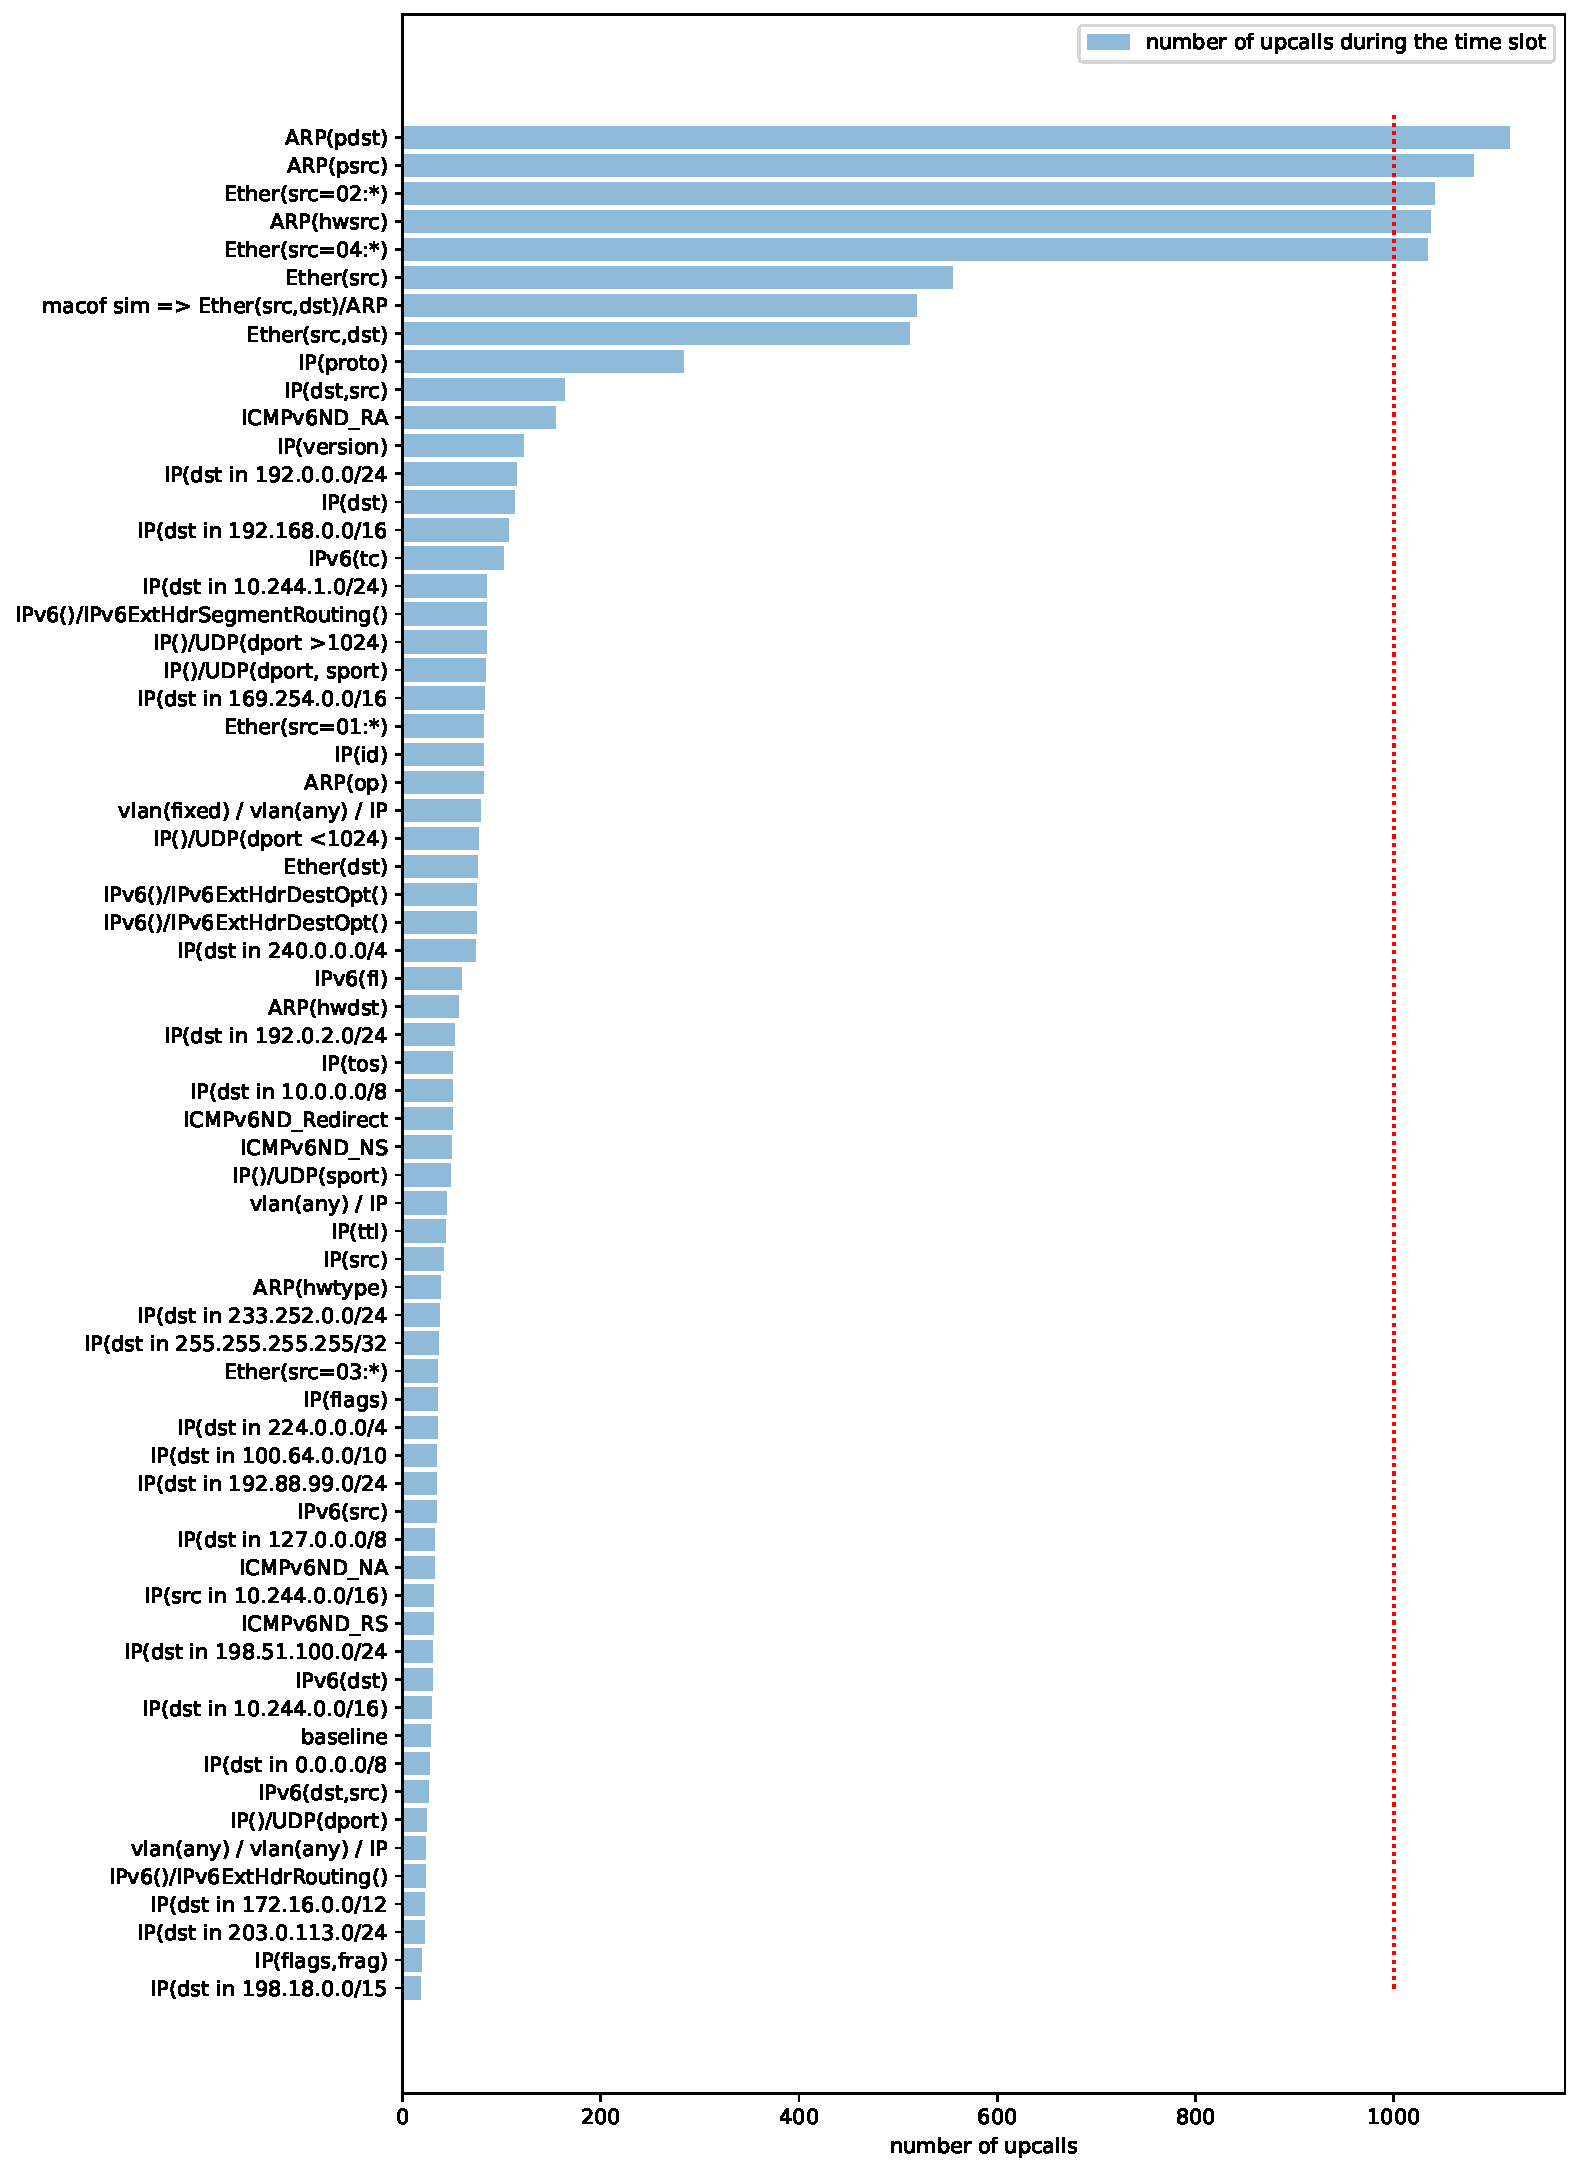
\includegraphics[width=.9\linewidth]{img/packet_fuzz.pdf}
    \caption{Number of upcalls generated by varying certain header fields in packets}
    \label{fig:plot-packet-fuzz}
\end{figure}

\Cref{fig:plot-packet-fuzz} shows the number of upcalls generated after sending 1000 crafted packets differing only in a value of a specified header field. We are interested in the peak of the plot, they signify packet types that consistently generate upcalls. The most significant being varying Ethernet source addresses and address fields in ARP packets.

\subsection{Ethernet source addresses}
\label{subsec:ethernet}

Varying the Ethernet source address in the unicast range (the least significant bit of the first byte has to be 1) generates new upcalls. The flow rules being inserted into the flow table are similar to the following example\footnote{dumped with \ident{ovs-dpctl dump-flows}}:

\begin{verbatim}
recirc_id(0),in_port(9),
    eth(src=04:6a:68:88:2b:eb),eth_type(0x0800),ipv4(frag=no),
    packets:0, bytes:0, used:never, actions:drop
\end{verbatim}

OVN has a feature called port security which can be enabled for logical switch ports. By enabling port security on a port, MAC spoofing is prevented and all packets with the wrong MAC address are dropped. OVN-Kubernetes enables this feature. The command \ident{ovn-nbctl list Logical\_Switch\_Port} prints configuration for all logical switch ports, including information about port security. The following snippet is part of the command's output, a description of the logical switch port used for our test pod called \ident{arch}.

\begin{verbatim}
_uuid               : cc7a2d01-52b4-4529-a026-55bf9d46dc56
addresses           : ["0a:58:0a:f4:01:05 10.244.1.5"]
dhcpv4_options      : []
dhcpv6_options      : []
dynamic_addresses   : []
enabled             : []
external_ids        : {namespace=default, pod="true"}
ha_chassis_group    : []
mirror_rules        : []
name                : default_arch
options             : {
    iface-id-ver="40c48294-7f78-4cc0-8a74-cffd9ecec647",
    requested-chassis=wsfd-netdev65.ntdv.lab.eng.bos.redhat.com
}
parent_name         : []
port_security       : ["0a:58:0a:f4:01:05 10.244.1.5"]
tag                 : []
tag_request         : []
type                : ""
up                  : true
\end{verbatim}

Quoting the OVN documentation, section about the port security option\footnote{The documentation calls it a column, because the configuration is stored in a database column}: \todo{link to https://www.man7.org/linux/man-pages/man5/ovn-nb.5.html}

\begin{quote}
    This column controls the addresses from which the host
    attached to the logical port (''the host'') is allowed to
    send packets and to which it is allowed to receive
    packets. If this column is empty, all addresses are
    permitted.

    Each element in the set must begin with one Ethernet
    address. This would restrict the host to sending packets
    from and receiving packets to the ethernet addresses
    defined in the logical port's port\_security column. It
    also restricts the inner source MAC addresses that the
    host may send in ARP and IPv6 Neighbor Discovery packets.
    The host is always allowed to receive packets to multicast
    and broadcast Ethernet addresses.
\end{quote}

The port security flow rules are added in OVN, in \ident{controller/lflow.c} in \href{https://github.com/ovn-org/ovn/blob/45bf9ed9dd2070a458bf384ce529e9ef62f26bd5/controller/lflow.c\#L3091-L3093}{function \ident{consider\_port\_sec\_flows()}}. OVN adds multiple OpenFlow rules into multiple flow tables to implement port security.

Because OVS's datapath flow rules are much simpler than OpenFlow flow rules, there is no 1-1 mapping between them. Moreso, the datapath flow rules allow only positive matches (see \cref{subsec:matching-algo}). They can not express negative matches. Therefore, when we send packets with varying MAC addresses, \ident{ovs-vswitchd} evaluates the packets against the OpenFlow rules and finds out that the packet should be dropped. The newly generated datapath flow rule checks for an exact match on the random MAC address and is not generic to match any other packets.

Looking at the problem from the other side, OVS's datapath is designed to assign packets to logical flows and execute the flow actions in as few instructions as possible. There are no precedence rules in the datapath flow table, the first matching rule is used and the order of insertion is not maintained. There are also only positive matches, no negative matches. Therefore, a single rule to drop all packets except for those with a given MAC address is impossible to construct.


% translation happens here https://github.com/openvswitch/ovs/blob/64cdc290ef441bc3b4c2cddc230311ba58bc31b3/ofproto/ofproto-dpif-xlate.c#L7769-L7778
% struct xlate_in https://github.com/openvswitch/ovs/blob/64cdc290ef441bc3b4c2cddc230311ba58bc31b3/ofproto/ofproto-dpif-xlate.h#L66
% struct xlate_ctx https://github.com/openvswitch/ovs/blob/64cdc290ef441bc3b4c2cddc230311ba58bc31b3/ofproto/ofproto-dpif-xlate.c#L195

\subsection{ARP packet fields}

ARP packets with varying hardware addresses behave the same as ordinary Ethernet packets with varying source hardware addresses because port security in OVN applies to them as well.

\subsection{Other types of packets}

OVN's documentation states that IPv6 Neighbour Discovery (ND) packets are also covered by the port security setting and we should be therefore able to observe the same behavior as with ARP packets. However, we did not generate any upcalls with the ND packets. There are two likely options why this is the case:

\begin{itemize}
    \item We did not configure the cluster properly for dual-stack networking with both IPv4 and IPv6. This is certainly a possibility, we did pay special attention to making IPv6 work. We focused only on IPv4.

    \item We might have crafted invalid IPv6 ND packets. While we believe they are correct, they have more validity requirements than simple IPv4 ARP packets and we might have made an error there.
\end{itemize}

Either way, we expect that IPv6 ND packets are also a potential problem and they should be checked as well when developing a fix.

\section{Impact of upcall heavy traffic}
\label{res:upcall-stress}

\subsection{Performance with unlimited resources}
\label{subsec:standard-behavior}

\begin{figure}
    \centering
    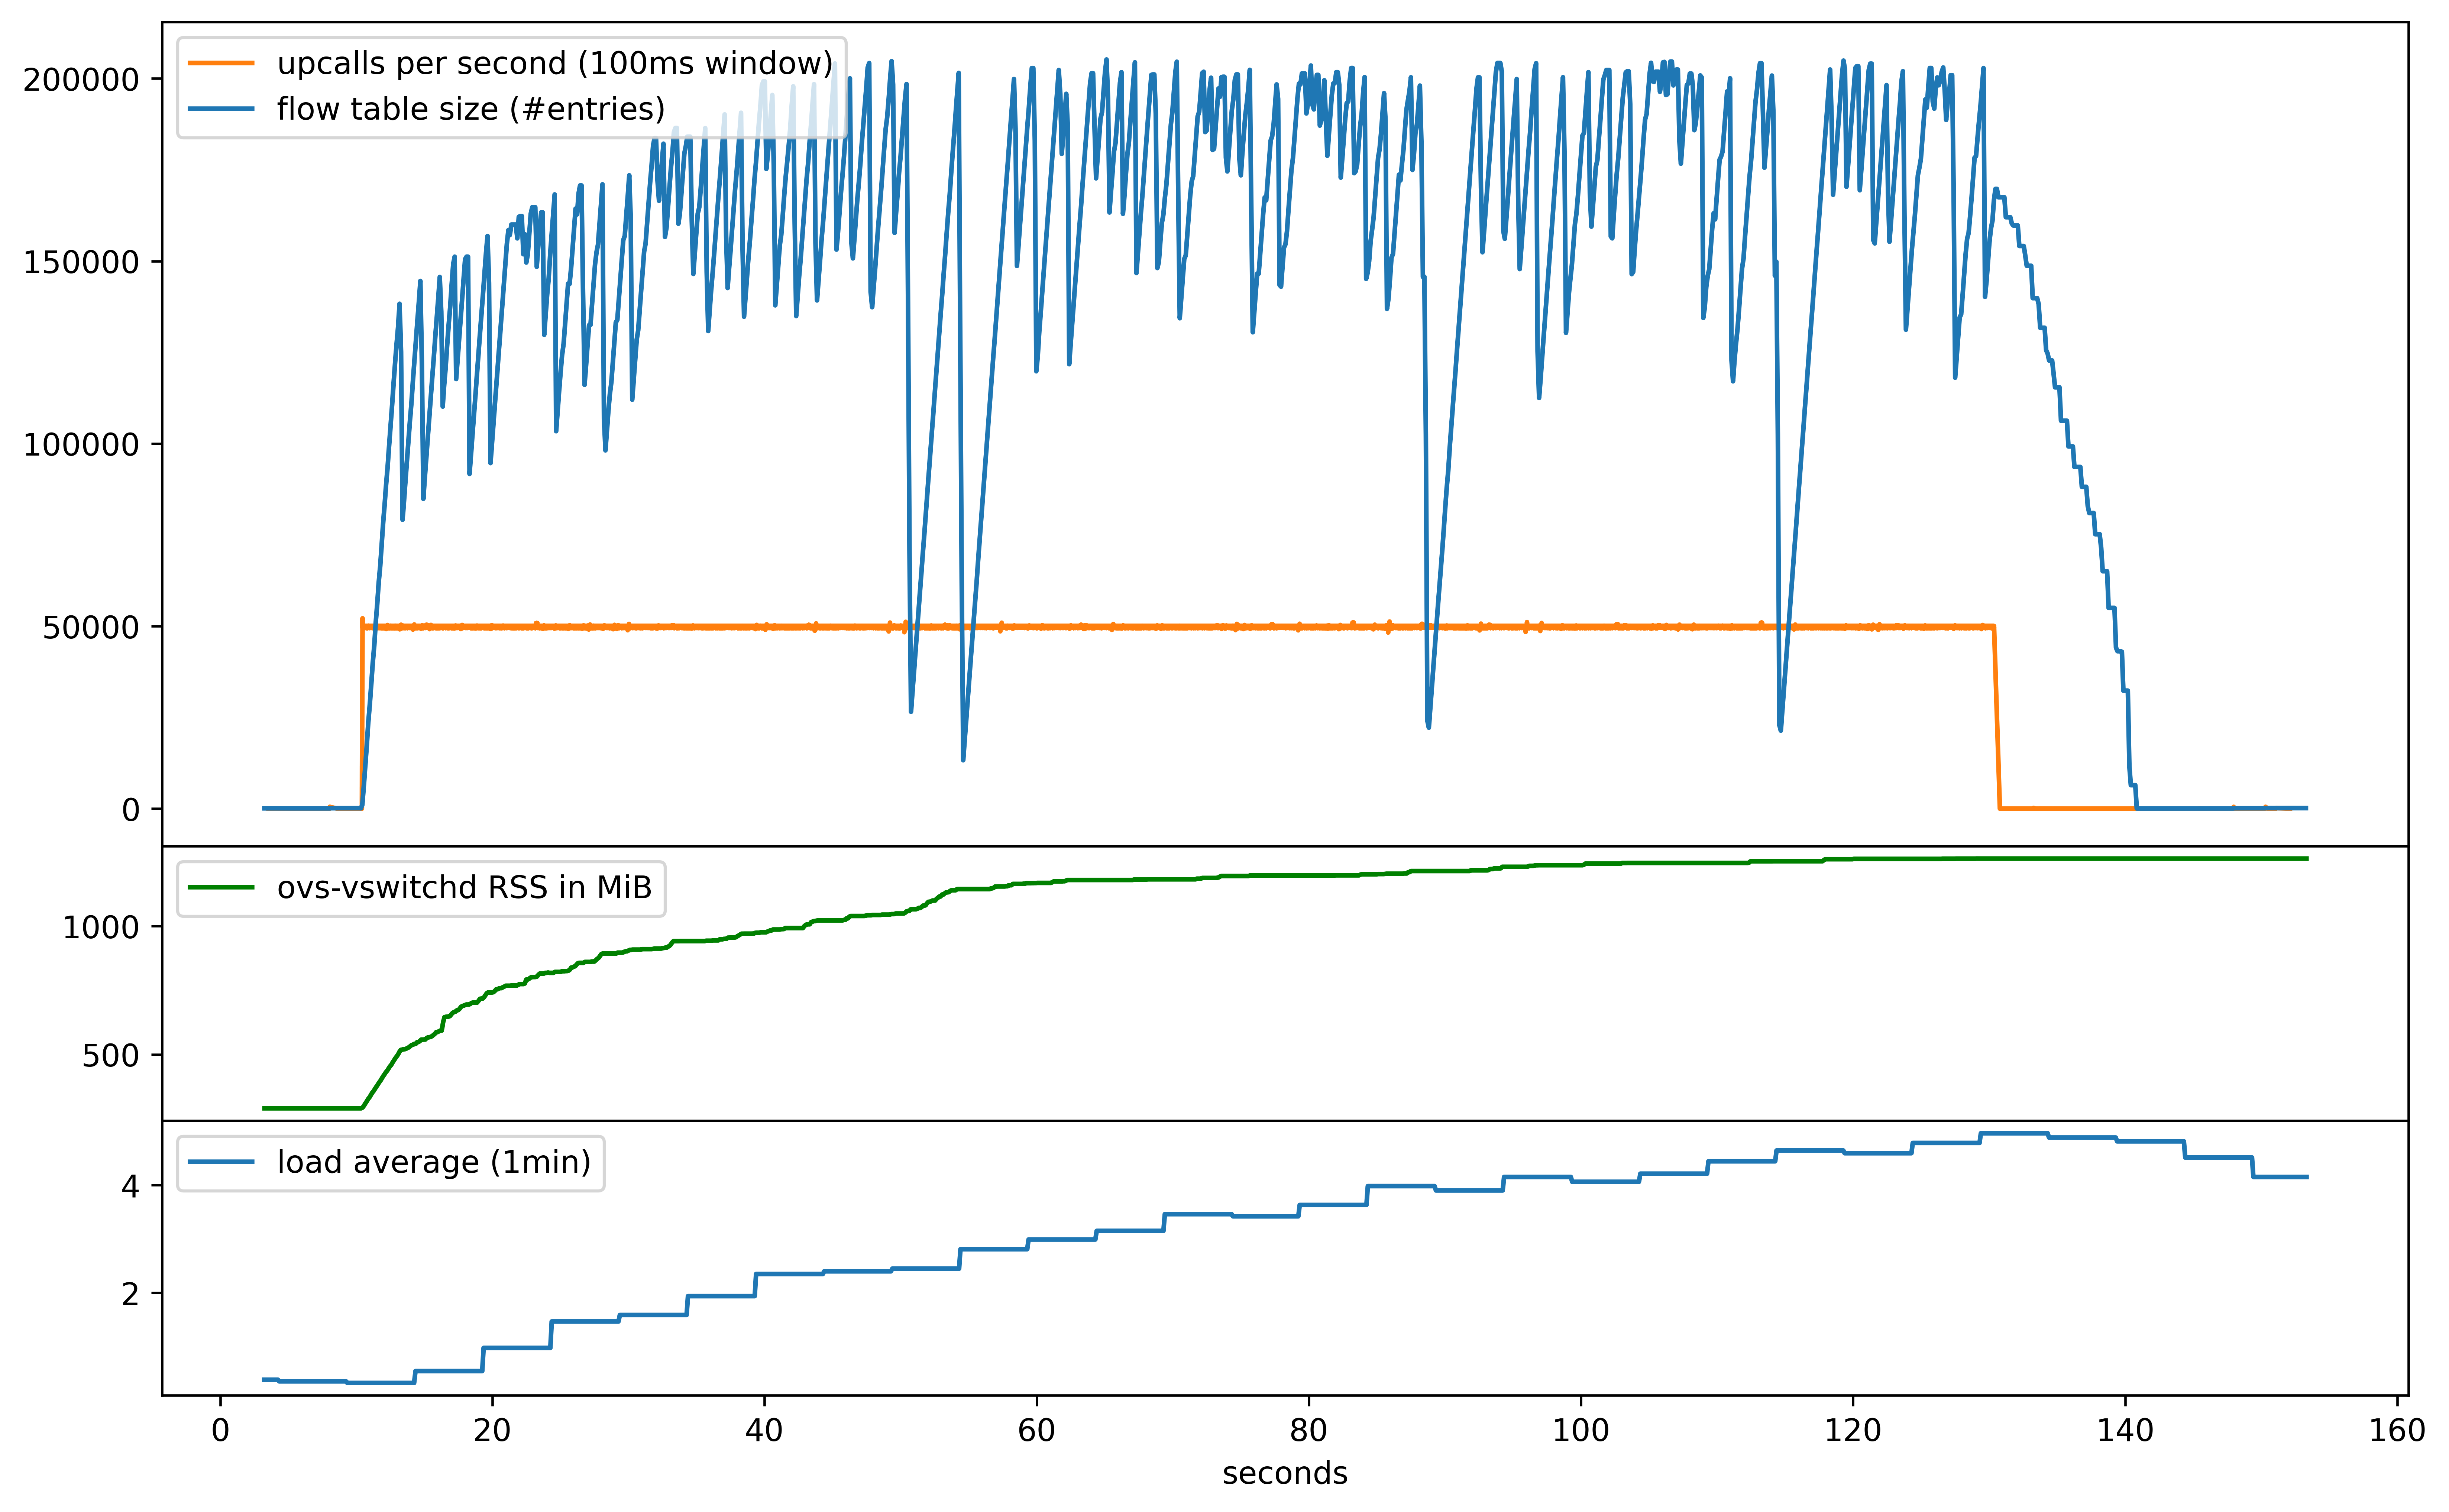
\includegraphics[width=.9\linewidth]{img/packet_flood_bare_50k.png}
    \caption{\ident{ovs-vswitchd} stressed with 50k upcalls per second}
    \label{fig:plot-packet-flood-bare-50k}
\end{figure}

\begin{figure}
    \centering
    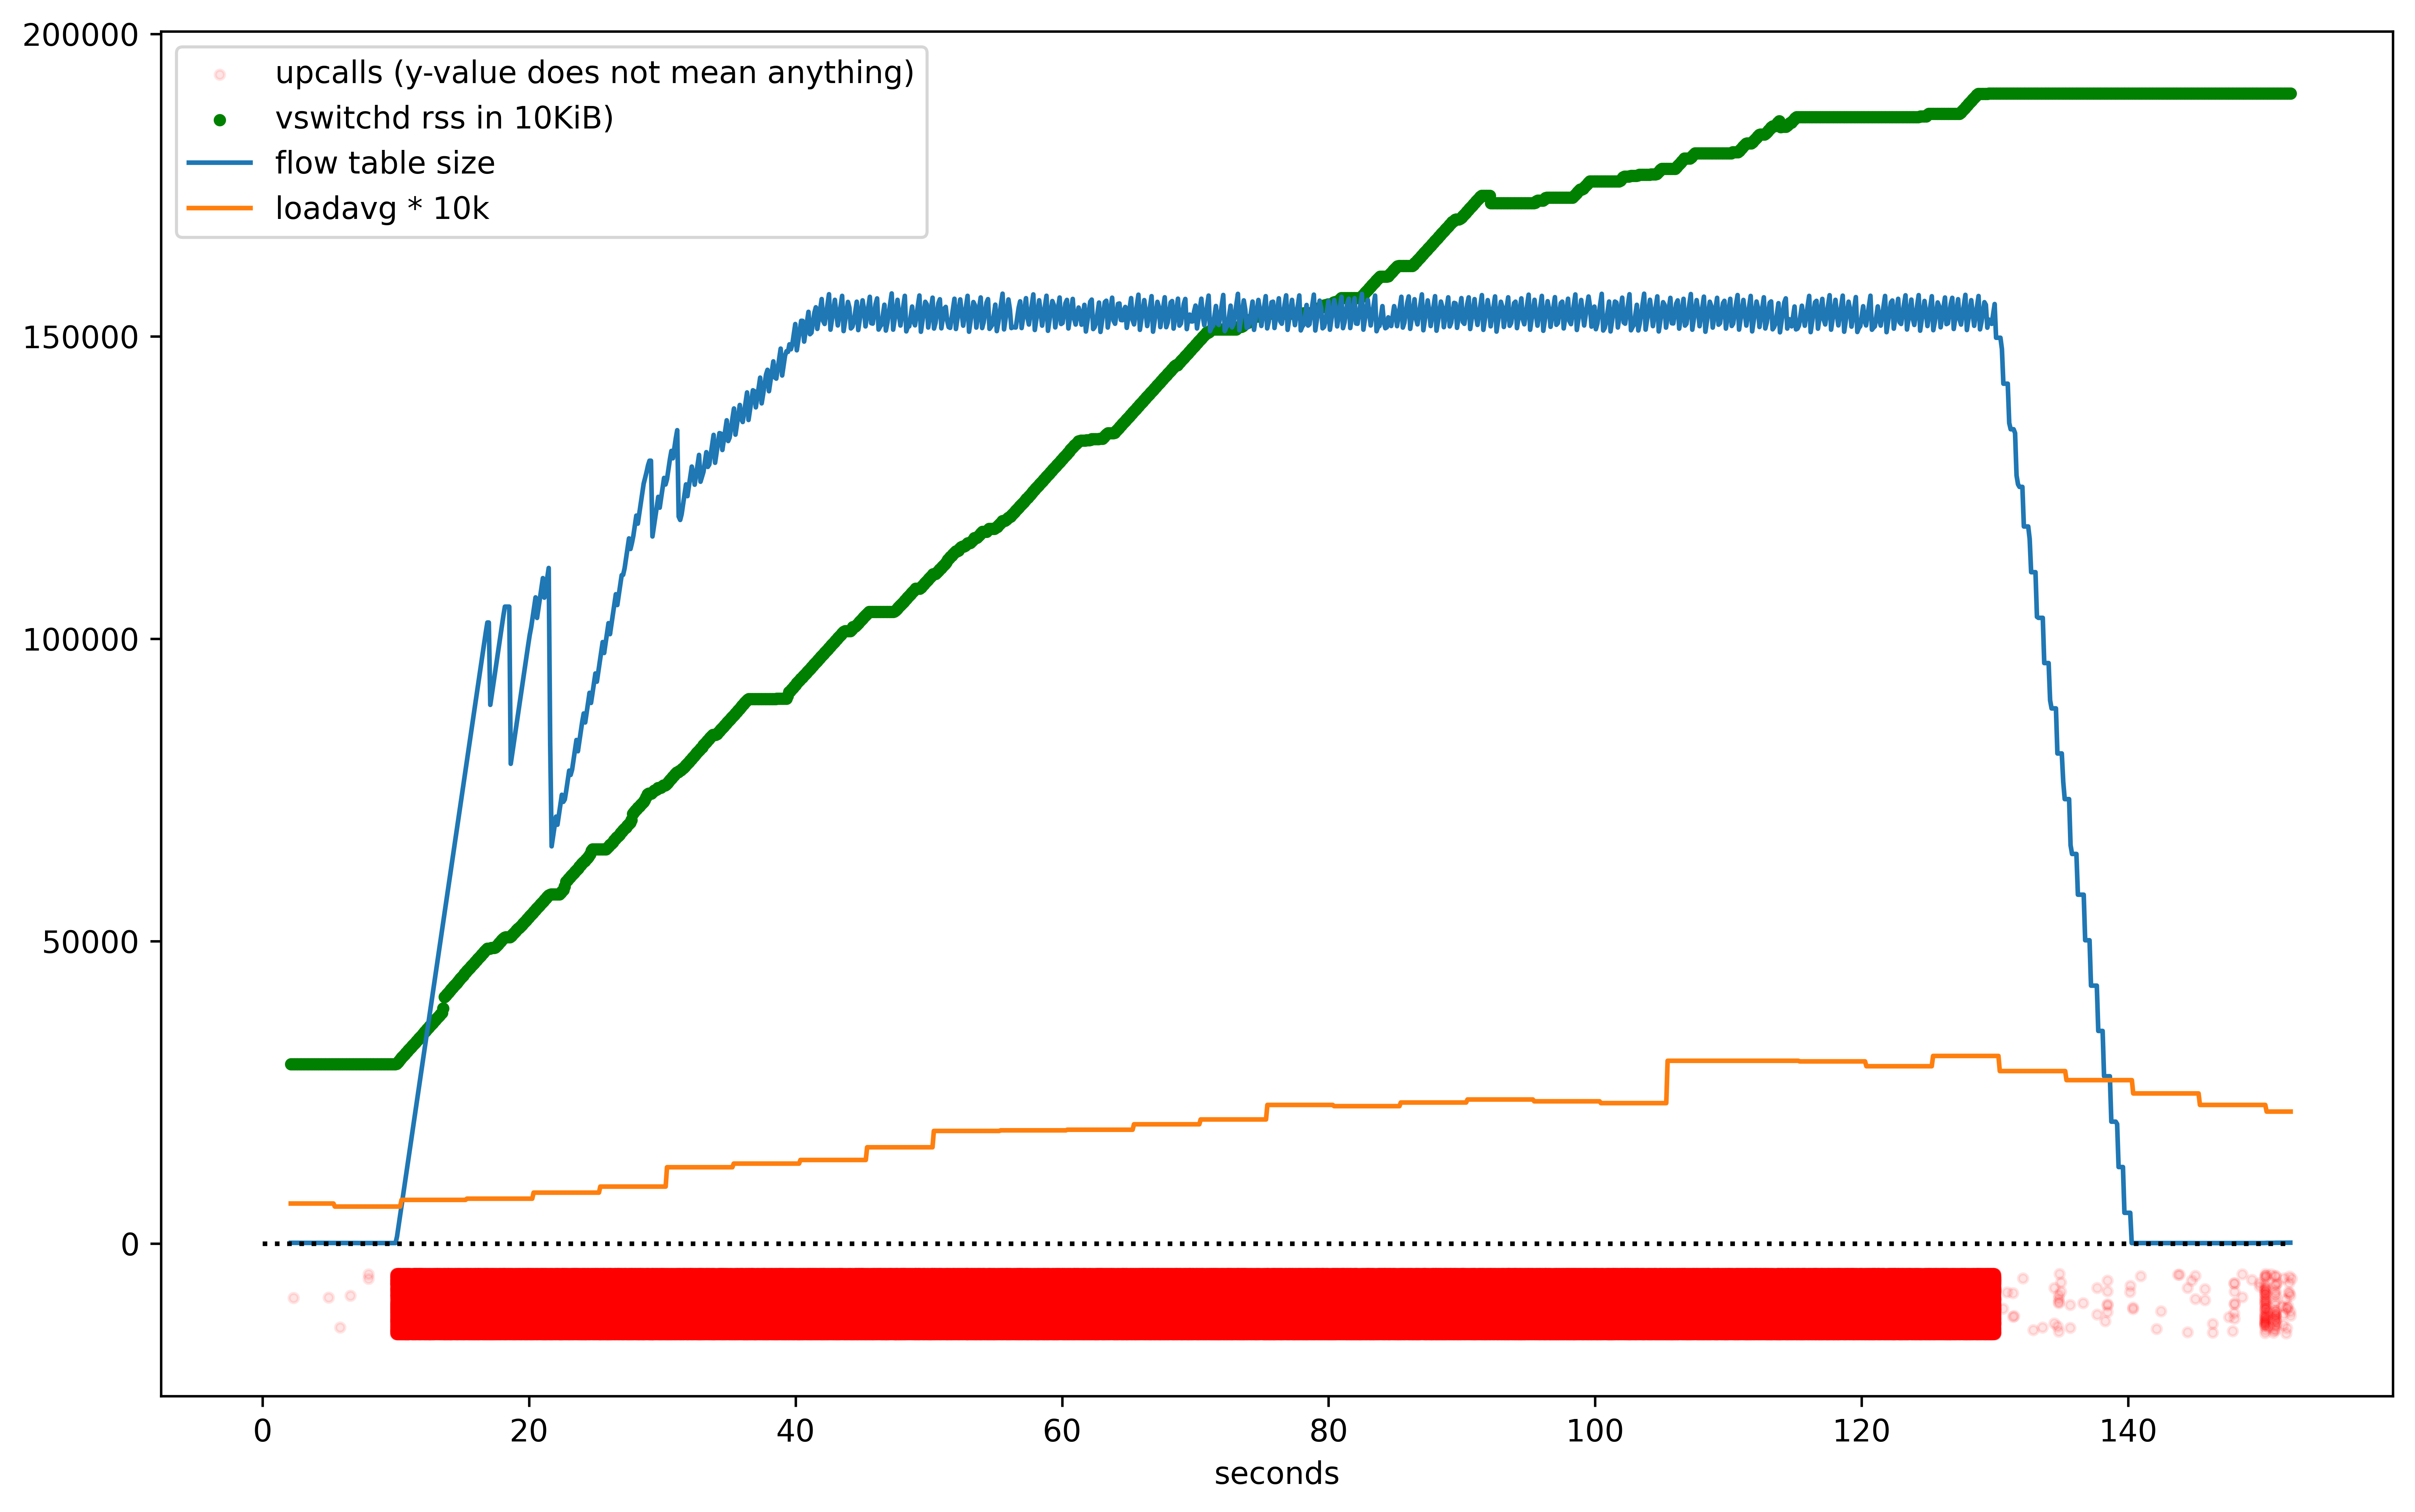
\includegraphics[width=.9\linewidth]{img/packet_flood_bare_15k.png}
    \caption{\ident{ovs-vswitchd} stressed with 15k upcalls per second}
    \label{fig:plot-packet-flood-bare-15k}
\end{figure}

\paragraph{Flow table size}
\Cref{fig:plot-packet-flood-bare-50k} and \cref{fig:plot-packet-flood-bare-15k} show recorded behavior of \ident{ovs-vswitchd} when stressed with significant number of upcalls. Assuming the 10-second flow rule timeout would be the only criteria for evicting flow rules, the flow tables should have reached 500k and 150k flow rules respectively. However, \ident{ovs-vswitchd} has a \href{https://github.com/openvswitch/ovs/blob/859071224c590207ca5e1f8723ffdef72ef7b512/ofproto/ofproto.h\#L310}{default limit of 200k flow rules} in the flow table which explains the lower-than-expected table size in \cref{fig:plot-packet-flood-bare-50k}. Moreso, the flow table size limit is dynamic based on measured system performance\todo{link to the future} and 200k is only a hard limit beyond which the table will never grow. The dynamic increase of the flow limit until the hard limit is reached is visible at the beginning of \cref{fig:plot-packet-flood-bare-50k}.

In both experiments, the flow table size fluctuates. With fewer upcalls, when only the timeout is at play, the fluctuations are small and can be explained by periodic timeout enforcement in the revalidator threads in \ident{ovs-vswitchd}. When the flow table size hits the 200k limit, an additional regulatory mechanism in the revalidator threads activates. Quoting a comment\footnote{\url{https://github.com/openvswitch/ovs/blob/474a179aff6c4199d8007910e3f79f000af9d659/ofproto/ofproto-dpif-upcall.c\#L2771-L2782}} from OVS's source code:

\begin{quote}
    In normal operation we want to keep flows around until they have
    been idle for 'ofproto\_max\_idle' milliseconds.  However:

    \begin{itemize}
        \item If the number of datapath flows climbs above 'flow\_limit', drop that down to 100 ms to try to bring the flows down to the limit.

        \item If the number of datapath flows climbs above twice 'flow\_limit', delete all the datapath flows as an emergency measure.  (We reassess this condition for the next batch of datapath flows, so we will recover before all the flows are gone.)
    \end{itemize}
\end{quote}

In other words, the revalidator thread checks flow rules in batches and whenever the flow table grows above the limit, a shorter eviction timeout is applied to the current batch. We hypothesize that the high amplitude of the fluctuations is caused by synchronization between multiple threads. There are multiple revalidator threads, each has its flow rule dump thread\footnote{\url{https://github.com/openvswitch/ovs/blob/474a179aff6c4199d8007910e3f79f000af9d659/ofproto/ofproto-dpif-upcall.c\#LL2751C16-L2751C16}} and the actual rule deletion is handled in the kernel after receiving a deletion command over a netlink socket which has an internal queue. We did not confirm nor disprove the hypothesis.

\paragraph{Upcalls}
In both \cref{fig:plot-packet-flood-bare-50k} and \cref{fig:plot-packet-flood-bare-15k}, the red dots at the bottom represent individual upcalls. We have randomized their position on the y-axis to improve legibility and better visualize upcall frequency.

Whenever our stress tool runs, the red bar becomes saturated and dense. Our tool tries to send packets in regular intervals, so the red bar should appear mostly homogeneous. At the end of the test, we report the results over the network and our tools are not perfectly synchronized, hence small upcall clusters at the end of the experiment are to be expected.

% aneb povidani o divnych upcallech, ktere uz vime, ze neni zajimave
% In \cref{fig:plot-packet-flood-bare-50k}, we can see a lot of upcalls happen before the stress test starts and they do not appear to be happening afterwards. We do not know what is causing it.\todo{FALSE! We know!} An ICMP and UDP latency test is running in the background (results in \todo{link do sekce s latenci}) as well as an SSH connection, but these packets should not be causing a significant number of upcalls. Furthermore, if it were caused by these packets, it should have continued after the stress test had finished. The other experiment shown here in \cref{fig:plot-packet-flood-bare-15k} has these upcalls both before and after the stress test. In other tests, we have also observed no extra upcalls.

\paragraph{System load}
Because our packet flooding tool is a single-threaded application, it directly contributes to the load averages only by a value of 1 or less. However, we observe a significantly higher load average in both recorded experiments, in \cref{fig:plot-packet-flood-bare-50k} and in \cref{fig:plot-packet-flood-bare-15k}. Except for our running experiment, the system is idle. Hence we attribute the additional system load to OVS. As we discussed before in \cref{subsec:ovs-tasks}, OVS uses multiple threads during normal operation. By default, the revalidator threads iterate over the whole flow table every 500 \si{\milli\second} and command the kernel to delete flow rules. The upcall handlers continuously translate OpenFlow rules to datapath rules and command the kernel to insert new flow rules. All of this busy work causes the extra system load.

Worryingly though, the additional system load is not attributed to the process causing it. In Kubernetes, a container can have a \href{https://kubernetes.io/docs/concepts/configuration/manage-resources-containers/}{resource limits assigned}. Flooding the system with upcalls from a resource-limited container would allow it to stress the system beyond its allowance. 

\paragraph{Memory usage}
\label{par:memory-usage}
In both \cref{fig:plot-packet-flood-bare-50k} and \cref{fig:plot-packet-flood-bare-15k}, the resident set size of \ident{ovs-vswitchd} increases and stabilizes at slightly less than 2GB. The allocated memory is never released and stays allocated even after the flooding stops. The used memory seems to be proportional to the flow table size.

Same as with the system load, memory usage bypasses resource accounting. A container or a VM with minimal resource allowance can use more resources than the system administrators configured.

\subsection{Impact on latency}

\begin{figure}
    \centering
    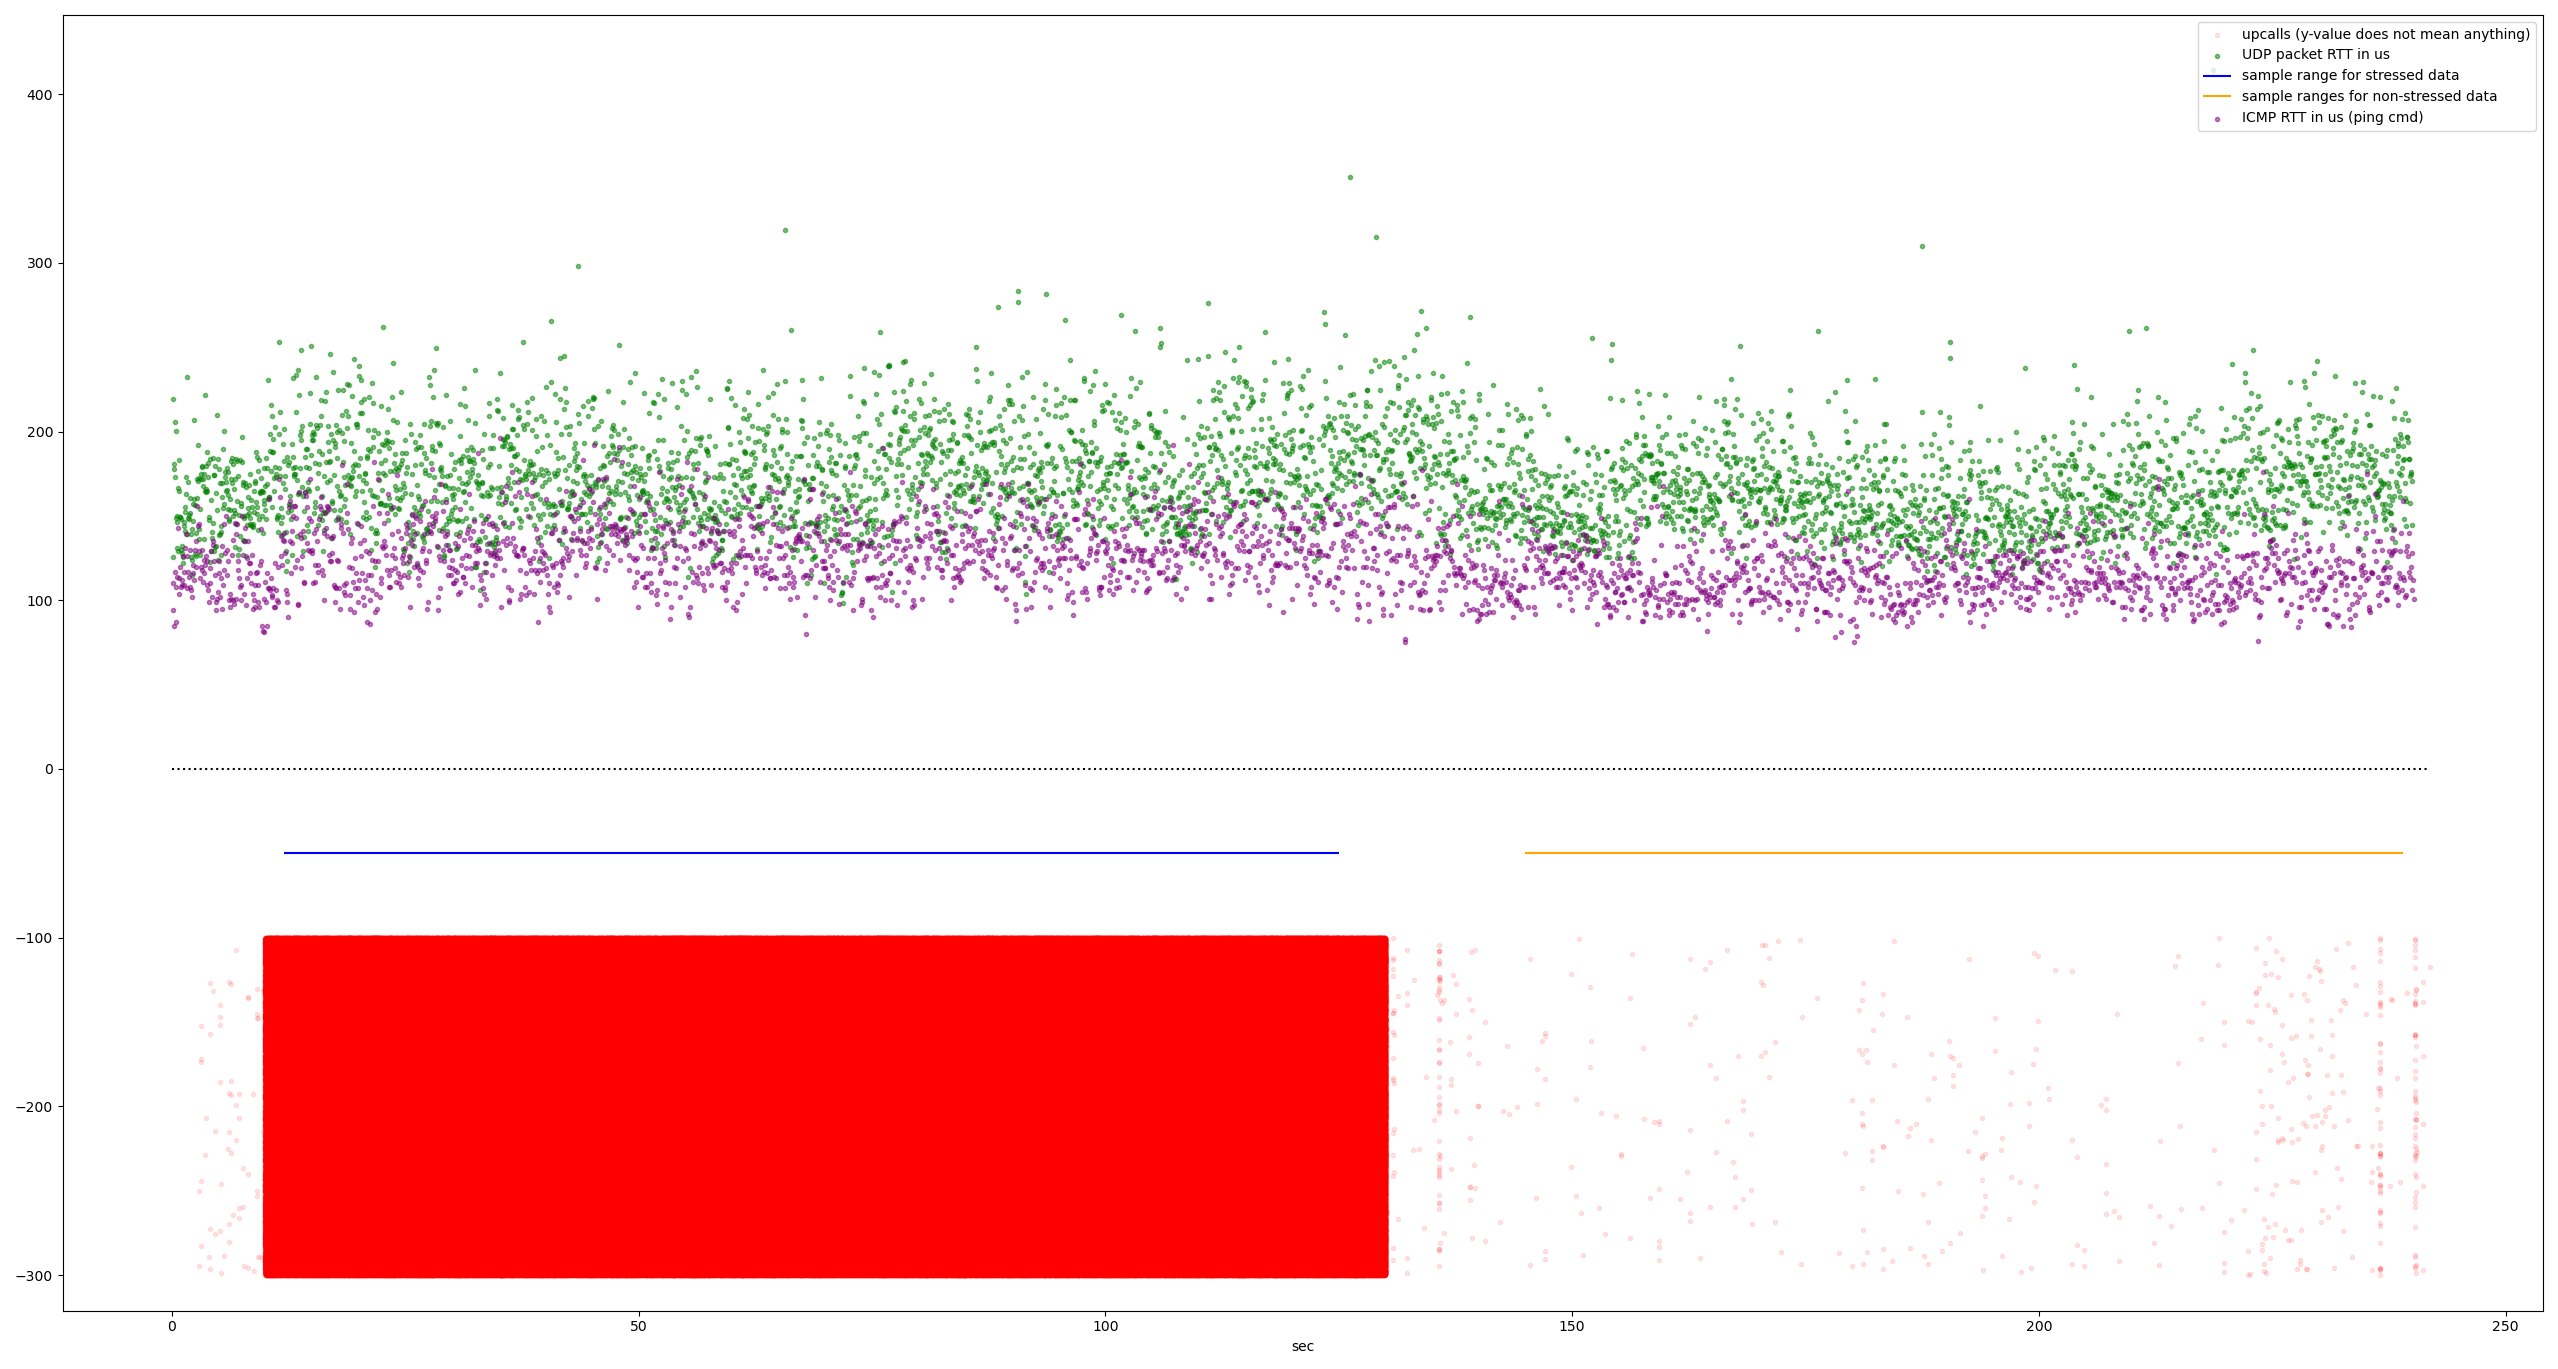
\includegraphics[width=.9\linewidth]{img/packet_flood_50k_latency.png}
    \caption{Round trip times during 50k upcalls/sec stress test}
    \label{fig:plot-packet-flood-50k-latency}
\end{figure}

\Cref{fig:plot-packet-flood-50k-latency} shows the results of a different run of the same experiment. The plot shows only the latencies measured from the \ident{victim} pod. The ICMP tests target the node IP address of \kb{1}, and the UDP tests target the node IP address of \kb{3}. The horizontal lines mark the ranges of samples used for a statistical test.

While there does not seem to be any practically significant difference between the stressed and non-stressed systems in the round-trip times, the difference is statistically significant. Considering only the UDP-based results, there are $2255$ samples in the stressed range with a mean value of $175980 \pm 1320$ \si{\nano\second}\footnote{$95\%$ confidence interval, assuming normal distribution}. The non-stressed range has 1876 samples and a mean value of $164404 \pm 1174$ \si{\nano\second}. The difference between the means is $11576$ \si{\nano\second}.

% stressed UDP latency
% shape: (9, 3)
% ┌────────────┬────────────┬───────────────┐
% │ describe   ┆ ts         ┆ latency_ns    │
% │ ---        ┆ ---        ┆ ---           │
% │ str        ┆ f64        ┆ f64           │
% ╞════════════╪════════════╪═══════════════╡
% │ count      ┆ 2255.0     ┆ 2255.0        │
% │ null_count ┆ 0.0        ┆ 0.0           │
% │ mean       ┆ 68.502237  ┆ 175980.142794 │
% │ std        ┆ 32.628849  ┆ 31963.391742  │
% │ min        ┆ 12.025217  ┆ 98250.0       │
% │ max        ┆ 124.979466 ┆ 762959.0      │
% │ median     ┆ 68.502056  ┆ 173259.0      │
% │ 25%        ┆ 40.238689  ┆ 155156.0      │
% │ 75%        ┆ 96.765862  ┆ 193006.0      │
% └────────────┴────────────┴───────────────┘
% (175980.14279379157, 174660.18226166346, 177300.10332591968)
% non-stressed UDP latencies
% shape: (9, 3)
% ┌────────────┬────────────┬───────────────┐
% │ describe   ┆ ts         ┆ latency_ns    │
% │ ---        ┆ ---        ┆ ---           │
% │ str        ┆ f64        ┆ f64           │
% ╞════════════╪════════════╪═══════════════╡
% │ count      ┆ 1876.0     ┆ 1876.0        │
% │ null_count ┆ 0.0        ┆ 0.0           │
% │ mean       ┆ 191.99893  ┆ 164404.665245 │
% │ std        ┆ 27.143008  ┆ 25925.644717  │
% │ min        ┆ 145.023486 ┆ 107262.0      │
% │ max        ┆ 238.975234 ┆ 495776.0      │
% │ median     ┆ 191.999098 ┆ 161704.5      │
% │ 25%        ┆ 168.52374  ┆ 146410.0      │
% │ 75%        ┆ 215.52409  ┆ 178624.0      │
% └────────────┴────────────┴───────────────┘
% (164404.66524520254, 163230.7366655189, 165578.5938248862)


\section{Performance when resource limited}

In \cref{subsec:standard-behavior}, we talked about extra memory and CPU usage of /ident{ovs-vswitchd}. The default containerized deployment of OVN-Kubernetes limits\footnote{https://github.com/ovn-org/ovn-kubernetes/blob/b982b8cadba939c55010829f61eb5ebe4fd90794/dist/templates/ovs-node.yaml.j2\#L84-L90} \ident{ovs-vswitchd} to 400 MiB of physical memory and two-tenths of a single CPU core. In the remainder of this section, when we write about limiting memory or CPU, we mean using Kubernetes to enforce the resource limit just as the default containerized deployment does it.

\subsection{Memory limit}
\label{subsec:memory}
We limited the memory usage of \ident{ovs-vswitchd}, leaving the CPU time unlimited. We used the default values for the memory limit, leaving us with the following configuration of the OVS container:

\begin{verbatim}
resources:
    requests:
        memory: 300Mi
    limits:
        memory: 400Mi
\end{verbatim}

When we flooded the system with upcalls, \ident{ovs-vswitchd} crashed without leaving any meaningful error message behind. During normal operations, everything seemed normal.

We tried to limit the number of flow rules using the following command:
\begin{verbatim}
ovs-vsctl set Open_vSwitch . other_config:flow-limit=10000
\end{verbatim}

The limit helps and when the upcall frequency is not too high (double or triple the limit), everything works. However, once we flood the network with even more packets, the flow limit is overshot and \ident{ovs-vswitchd} again crashes.

Our theory is that the crash happens during the revalidator dump phase, when \ident{ovs-vswitchd} makes a copy of all in-kernel flow rules in the userspace. This allocates more memory than allowed and the container is subsequently terminated:

\begin{quote}
    A Container can exceed its memory request if the Node has memory available. But a Container is not allowed to use more than its memory limit. If a Container allocates more memory than its limit, the Container becomes a candidate for termination. If the Container continues to consume memory beyond its limit, the Container is terminated. If a terminated Container can be restarted, the kubelet restarts it, as with any other type of runtime failure.
    \todo{link source https://kubernetes.io/docs/tasks/configure-pod-container/assign-memory-resource/}
\end{quote}

The decreased flow limit in the configuration of OVS does not help much to prevent crashes, because we can inject too many flows in between the revalidator thread runs (we can inject about 100k flow rules in 500ms, \ident{ovs-vswitch} crashes even with less).

\subsection{CPU limit}
\label{subsec:cpu-limit}

When CPU bound, \ident{ovs-vswitchd} does not crash. It tries to do the opposite and \href{https://github.com/openvswitch/ovs/blob/e3ba0be48ca457ab3a1c9f1e3522e82218eca0f9/ofproto/ofproto-dpif-upcall.c\#L1031-L1041}{dynamically change the datapath's flow rule limit} based on the revalidator thread's performance:

\begin{verbatim}
duration = MAX(time_msec() - start_time, 1);
udpif->dump_duration = duration;
if (duration > 2000) {
    flow_limit /= duration / 1000;
} else if (duration > 1300) {
    flow_limit = flow_limit * 3 / 4;
} else if (duration < 1000 &&
            flow_limit < n_flows * 1000 / duration) {
    flow_limit += 1000;
}
flow_limit = MIN(ofproto_flow_limit, MAX(flow_limit, 1000));
\end{verbatim}

We can see the effect of this code in \cref{fig:packet-flood-limited}. The red dots (not upcalls) signify the dynamic flow limit. The horizontal lines going to the left of the dots signify the time the revalidator run took. We can see how a long revalidator run leads to a decreased flow limit.

\begin{figure}
    \centering
    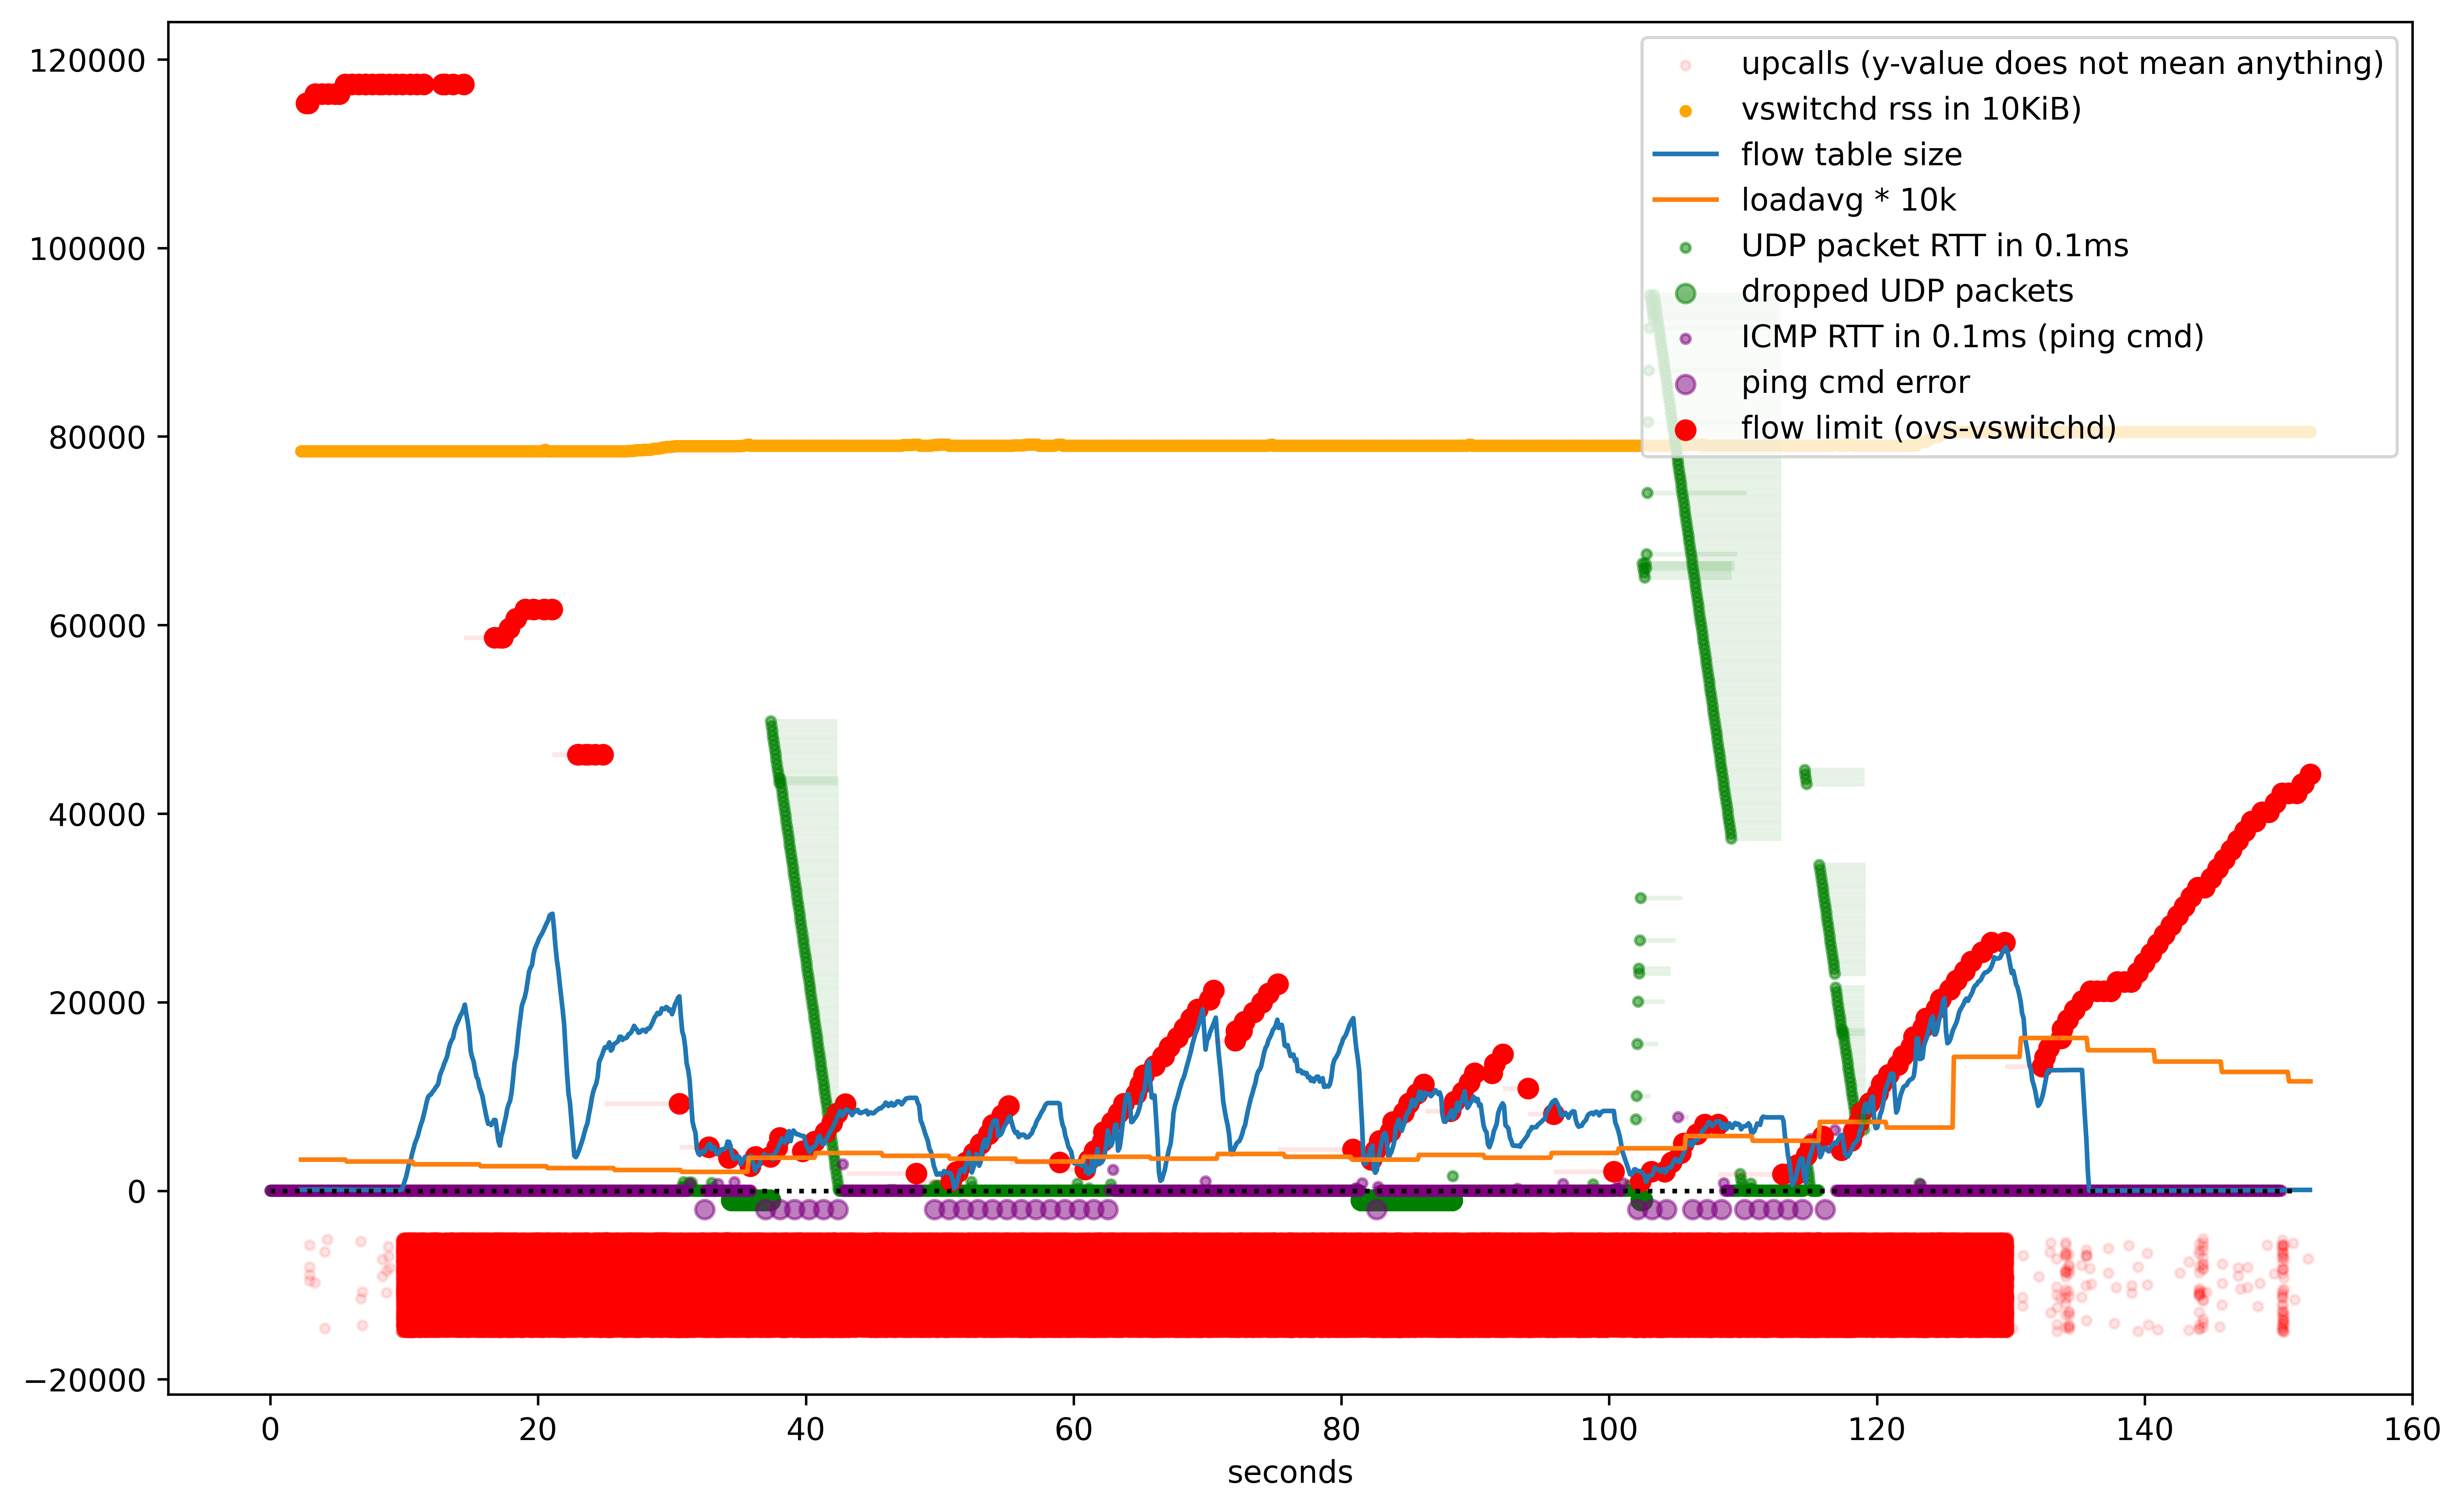
\includegraphics[width=.9\linewidth]{img/packet_flood_limited_resources_50k.png}
    \caption{5k upcalls/sec stress test}
    \label{fig:packet-flood-limited}
\end{figure}

 When compared to the previous experiments:

\begin{itemize}
    \item The rate of upcalls is only $5000$ per second, one-tenth of the experiments before.
    \item Memory usage stays almost constant.
    \item Load average (1 minute) peaks at the value 2\todo{this is weird, can we get a better run?}, but stays below 1 most of the time.
    \item The size of the datapath flow table varies a lot more. We can see the same higher frequency variations as before, but now they are combined with lower frequency variations created by the dynamically changing flow limit.
    \item Latency measurements are added to the plot (beware of the unusual units). They are the same as when we talked about latency before, now combined in a single experiment. The highest round-trip-time observed is around 10 seconds long. Sometimes, sending a packet completely fails (indicated by thicker dots below the number line).
\end{itemize}

The extremely high round-trip times can be explained by the upcall buffer queues. When the revalidator threads and other tasks use most of the available resources, the handler threads might not get scheduled and the packets in upcalls are buffered until the handler threads run again.

\paragraph{Crashes}
\label{par:cpu-crashes}
Surprisingly, \ident{ovs-vswitchd} also crashes if we flood the system with packets without any limit (i.e. roughly 210k packets per second). A possible explanation could be overflow somewhere in the handler thread queues, but this is a complete guess as there are no log messages left.

\subsection{Overloading \ident{ovs-vswitchd} without resource limits}

The crashes of \ident{ovs-vswitchd} with CPU limits led us to search for a possibility of a crash when overloaded without resource constraints. We tried to spawn multiple instances of our packet flooding tool. On the 28-core dedicated test servers, we did not manage to crash \ident{ovs-vswitchd} with anywhere between 1 and 80 instances of our stress tool.

We believe that \ident{ovs-vswitchd} is safe from crashes as long as it runs without resource constraints. On our experimental clusters, \ident{ovs-vswitchd} is automatically configured as a higher priority process than the ordinary processes and therefore it gets enough CPU time. But even if we manually decrease the priority to the same level or below ordinary processes, \ident{ovs-vswitchd} does not crash.